%
% ==========      Text pages
%

\textpages
 
% ========== Chapter 1
 
\chapter {Introduction}

\section{Weak Interactions and Rare Event Searches as a Key to New Physics}
Since its introduction by Wolfgang Pauli in 1930, the neutrino has been allowing physicists to patch together theories and experiments that did not quite align. At the time, the theories in question were the conservation of energy and angular momentum; beta decay observations seemed to violate these key principles, showing that the outgoing electron could carry off a range of energies up to the Q-value of the decay. With the addition of a light, spin-1/2, neutral particle, beta decay was explained as a three-body process, and the conservation laws could be saved. Though the newly-proposed particle evaded detection for over twenty years, it was eventually observed in 1956 \cite{Cowan1956}, vindicating Pauli's "desperate remedy." \cite{Pauli1930}

As the properties of neutrinos become better understood, they continue to play this role, pulling our theories back from the brink of incorrectness-- the ``solar neutrino problem" was eventually resolved by the introduction of neutrino flavor oscillations and neutrino mass. \cite{PDG2014} Other proposed aspects of neutrino physics could reveal neutrinoless double beta decay, a lepton number-violating process that could explain the source of matter/anti-matter imbalance in the universe. If this decay were observed, the neutrino would be a Majorana particle (meaning that it is its own antiparticle), explaining the origin and smallness of the neutrino masses.

The weak sector as a whole could also contain other as-yet undiscovered fixes for unexpected observations. The ``missing mass" apparent in galactic rotation curves and the cosmic microwave background, among other observations, could be explained by the discovery of some form of ``dark" (i.e. neutral) matter. A leading candidate is a class of particles called ``WIMPs" (Weakly-Interacting Massive Particles), which could be observed via WIMP-nuclear scattering, a weak force interaction. 

Aside from their potential to discover extensions to the standard model, weak-sector observations should reveal rare standard-model interactions. Two-neutrino double beta decay, for instance, was proposed in 1935, but remained undetected until 1987 \cite{Moe1987}. In today's generation of neutrinoless double-beta decay experiments, however, it is one of the most significant sources of background events. A process that remains unobserved is coherent neutrino-nuclear scattering. Modern detectors and low-background techniques have finally put an observation of this process within reach. 

\subsection{Neutrino Oscillations and Mass}
The neutrinos are standard-model fermions that interact only via gravity and the weak force. 

The weak interaction proceeds via two classes of vertex, called the neutral and charged currents. The Feynman diagrams for these processes are seen in Fig.~\ref{weak_diagrams}. In the charged current interactions, the standard model requires charge and lepton number conservation. Therefore, a charged lepton (i.e. the electron, muon, or tau, or their antiparticles) participates in the interaction, and the (anti-)neutrino always occurs with the W+(-) boson. There are (at least) three neutrino flavors, corresponding to the three charged leptons, which form a basis of flavor eigenstates. They are created in these eigenstates-- in a charged current interaction emitting an electron, for instance, the standard model requires that an electron anti-neutrino is also created. 

\begin{figure}[h]
\hfil 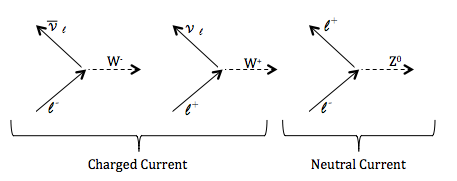
\includegraphics[width = .80\textwidth]{/Users/jgruszko/Documents/Thesis/Images/Ch1/WeakDiagrams.png} \hfil
\caption{The primitive vertices of the Feynman diagrams for weak interactions between leptons in the standard model. Equivalent vertices exist for the quarks. \cite{PDG2014}}
\label{weak_diagrams}
\end{figure}

Neutrino oscillation arises because the neutrinos have mass eigenstates (called 1, 2, and 3) that are different from their flavor eigenstates. Therefore, as they propagate in mass/momentum eigenstates, their flavors change according to the PMNS mixing matrix, a unitary matrix that connects the two bases.  The differences in the masses squared of the states also appears in the oscillation probabilities, so these values can be found from neutrino oscillation experiments. The sign of m$_{2,3}$$^{2}$, however, is currently unknown, leading to what are called the ``normal" and ``inverted" cases of the neutrino mass hierarchy, as seen in Fig.~\ref{mass_hierarchy}. 

\begin{figure}[]
\hfil 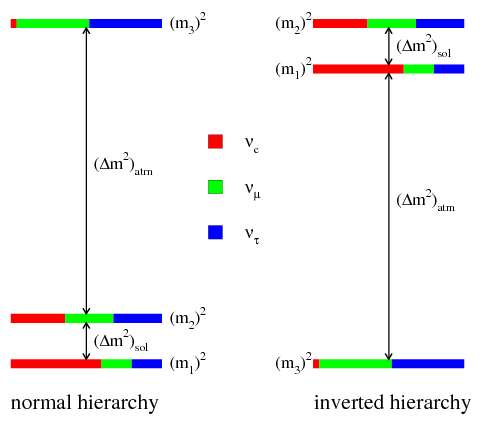
\includegraphics[width = .40\textwidth]{/Users/jgruszko/Documents/Thesis/Images/Ch1/MassHierarchy.png} \hfil
\caption{The two possible cases of the neutrino mass hierarchy \cite{Hewett2012}}
\label{mass_hierarchy}
\end{figure}

Additionally, the overall neutrino mass is not known. The lowest limits, derived from the shape of the $^{3}$He $\beta$-decay spectrum, give $m_{\bar{\nu}_{e}} < 2.3~eV$ \cite{Eitel2005}. More stringent limits, below $0.23~eV$, have been derived from cosmic microwave background observations \cite{PlanckXVI_2013}, but these values are highly model-dependent. The KATRIN experiment plans to directly probe masses down to $m_{\bar{\nu}_{e}} \sim 0.20~eV$ \cite{KATRIN2015}

\subsection{The Neutrino- Majorana or Dirac?}
Because neutrino oscillations have been observed, it is clear that neutrinos have non-zero mass. Minimalistic Higgs models, however, require fine-tuning, unnaturally leaving the neutrino mass about six orders of magnitude smaller than the masses of the other standard model particles. Any mechanism for neutrino mass that avoids this unnaturalness must come from an extension to the standard model. One possibility, called the ``see-saw mechanism," relies on the addition of a Majorana mass term \cite{Supergravity1979}. With the introduction of this term, there are no longer (non-interacting) right-handed neutrinos and left-handed antineutrinos. Instead, the neutrino and antineutrino are opposite-helicity states of the same Majorana particle. The Majorana mass term would contribute to the overall observed neutrino mass along with remaining Dirac mass terms, and could lead to lepton-number violating interactions. These interactions also allow a mechanism by which baryogenesis could be possible, leading to matter/anti-matter imbalance in the observable universe. \cite{DiBari2012}  

\subsection{Neutrinoless Double Beta Decay}
The most promising process by which to discover the nature of the neutrino is neutrinoless double beta decay. In standard-model two neutrino double-beta decay, a nucleus that contains an even number of nucleons is energetically forbidden from decaying via single beta-decay. Instead, two beta decays occur, leading to the emission of two electrons and two electron anti-neutrinos. In the neutrinoless version of this process the anti-neutrino is exchanged as a virtual particle-- it functions as an outgoing antineutrino for one of the beta decays, and as an incoming neutrino for the other decay. Thus, no neutrinos are seen in the final state:
$$M(A, Z) \rightarrow D(A, Z+2) + 2 e^{-},$$
 and all of the energy of the decay is carried by the electrons. Due to momentum conservation, the nucleons carry a negligible amount of the energy. This decay relies on the non-conservation of lepton number, which is allowed in the Standard Model, though it has not yet been observed, on the Majorana nature of the neutrino, and on the fact that the neutrino is in a mixed helicity state. Because of the last consideration, the effective size of the Majorana mass term, 
 $$\langle m_{\beta\beta} \rangle = |\sum\limits_{i=1}^3 U^2_{ei}m_i|,$$
 where $U_{ei}$ is the mixture of neutrino mass eigenstates $i$ in the electron neutrino, appears in the $0\nu\beta\beta$ rate:
 $$(T_{1/2}^{0\nu})^{-1} = G^{0\nu}|M_{0\nu}|^{2}\left(\frac{\langle m_{\beta\beta} \rangle}{m_e}\right)^2 .$$
 $G^{0\nu}$ is a phase space factor, $M_{0\nu}$ is the nuclear matrix element, and $m_e$ is the electron mass. Because they contribute to $m_{\beta\beta}$, both the overall neutrino mass and the mass hierarchy can contribute to the observed rate, as seen in Fig.~\ref{0nBBrate}. The experimental signature of such a decay would be a delta-peak in energy at the endpoint of the two-neutrino mode spectrum, as in Fig.~\ref{0nBBspectrum}.
 
 \begin{figure}[h]
 \centering
    \begin{subfigure}[b]{.40\textwidth}
      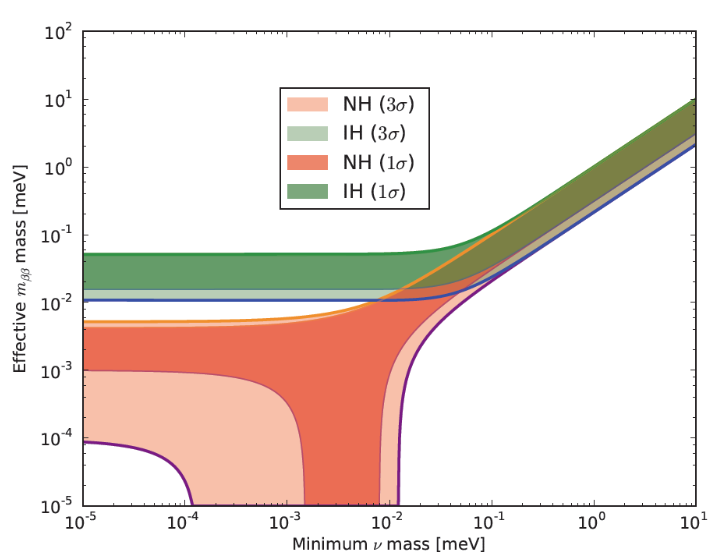
\includegraphics[width =\textwidth]{/Users/jgruszko/Documents/Thesis/Plots/Ch1/0nBB_Rate.png}
       \caption{$m_{\beta\beta}$, and therefore the $0\nu\beta\beta$ rate, depend on the neutrino mass hierarchy and the overall mass scale \cite{ZuberINT2015} .}
        \label{0nBBrate}
        \end{subfigure}   
         \hfil
        \begin{subfigure}[b]{0.4\textwidth}
      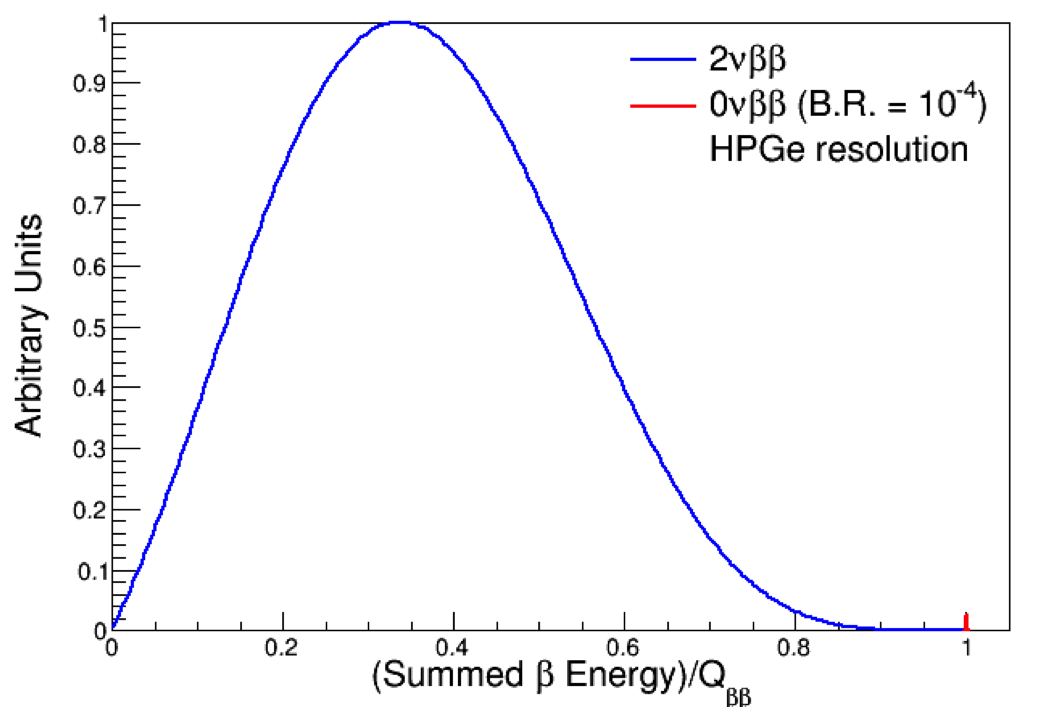
\includegraphics[width =\textwidth]{/Users/jgruszko/Documents/Thesis/Plots/Ch1/DoubleBetaEnergy.png} 
      \caption{The experimental signature of $0\nu\beta\beta$ decay as it would appear in \iso{76}{Ge}. Plot courtesy of Jason Detwiler.}
      \label{0nBBspectrum}
    \end{subfigure}   
\end{figure}
 
\subsubsection{Observing 0$\nu\beta\beta$}
Current limits set the $0\nu\beta\beta$ half-life to greater than $10^{25}$ years \cite{EXO2014}. To observe such a rare decay, backgrounds of $0\nu\beta\beta$ experiments must be extremely low, and the mass of source material must be as large as possible. Several strategies are commonly used by the $0\nu\beta\beta$ community. 

Some are determined solely by the choice of source material:
\begin{itemize}
\item Choice of Q Value: The higher the Q-value of the $0\nu\beta\beta$ decay in some material, the less background contamination will occur in the signal region. While incomplete energy collection, Compton scattering, and other processes can cause background events to appear at energies below the peak value of the decay, events generally cannot gain energy by any process. 
\item Enrichment: Source materials often have to be enriched in the $0\nu\beta\beta$ isotope to allow for higher source masses without increasing backgrounds. The ease and expense of this process varies widely depending on the material, as does the need for enrichment.
\item Favorable Matrix Elements: $M_{0\nu}$ varies between isotopes; a favorable rate could increase the $0\nu\beta\beta$ rate. However, different calculation strategies lead to variation in these values that is on the order of the difference between isotopes. See \cite{Simkovic2009} for further discussion. 
\item Low $2\nu\beta\beta$ Rate: The resolution of any detector is imperfect, so events from the high-energy tail of the $2\nu\beta\beta$ will contribute to the background. The $2\nu$ rate is unrelated to the $0\nu$ rate.
\end{itemize} 
Unfortunately, there is no ``magic bullet" isotope for $0\nu\beta\beta$ that has all the favorable properties. 

Other strategies for background reduction are affected by the detector technology used and the design of the experiment:
\begin{itemize}
\item Source as Detector: Using the same material for both source and detector increases efficiency and makes it easier to increase source mass without increasing backgrounds.
\item Surface Event Rejection and Fiducial Volume Cuts: Generally, the bulk of the source/detector material is low in background, and most background events are from surface contamination, external sources or other components of the experiment. Detection strategies that allow surface events to be removed from the data set can often reduce backgrounds by taking advantage of self-shielding.
\item Multi-Site Rejection and Particle Identification: Many backgrounds are from $\gamma$ and $\alpha$ particles. The former often lead to multi-site interactions, while $0\nu\beta\beta$ is by its nature a single-site process, since electrons have much a shorter mean-free-path than photons in detector materials. If the detector can distinguish between multi-site and single-site interactions, backgrounds can be reduced. $\alpha$ backgrounds can be distinguished from $e/\gamma$ interactions in many two-energy-channel detectors, like time projection chambers and scintillating bolometers, and similarly reduced. 
\item High Resolution: Higher resolution makes background events easier to identify and shrinks the region of interest (ROI) for $0\nu\beta\beta$ decay, making background requirements less stringent.
\item Low Thresholds: Low energy thresholds are not required, but can allow better identification of high-energy backgrounds through timing cuts that search for L- and K-shell decay peaks of short-lived intermediate states of certain background decays. 
\item Large Overburden: All competitive $0\nu\beta\beta$ decay experiments are housed underground, to decrease the rate of cosmic-ray backgrounds and cosmogenic activation of detector materials. 
\end{itemize}

A controversial claim of observed $0\nu\beta\beta$ in \iso{76}{Ge} was published by Klapdor-Kleingrothaus et. al \cite{KK2001} in 2001. The current generation of experiments aims to evaluate this claim at high confidence and evaluate techniques for future experiments. The goal of the next generation of experiments is to search the entire inverted-hierarchy region, which requires 1 tonne of source material, given reasonably achievable backgrounds. See Fig.~\ref{IH_Discovery}. 

\begin{figure}[h]
\hfil 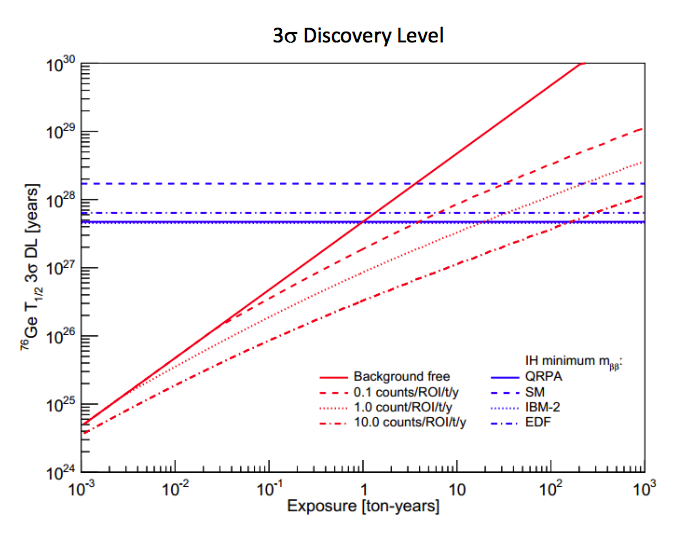
\includegraphics[width = .60\textwidth]{/Users/jgruszko/Documents/Thesis/Plots/Ch1/IH_Discovery.png} \hfil
\caption{The background requirements and exposure needed for $3\sigma$ discovery-level observation of $0\nu\beta\beta$ decay, assuming the inverted hierarchy. Plot courtesy of Jason Detwiler.}
\label{IH_Discovery}
\end{figure}


\subsection{Dark Matter}
Extensive evidence has shown that some as-yet-unknown neutral particle is contributing to the structure of the universe on galactic to cosmological scales. 

The first indications that there might be ``missing mass" came from Doppler-shift measurements of the velocities of edge-on spiral galaxies at different radii. Based on evaluations of luminous matter density, the orbital velocity is expected to decrease outside of the dense core of the disk. Instead, the orbital velocities remain constant out to radii much larger than the size of the luminous disk. \cite{Corbelli2000}  Modified theories of gravity were considered as a potential explanation for the anomaly, along with potential standard-model sources of mass such as small black holes, neutrinos, and unobserved brown dwarf stars, but these explanations have fallen out of favor as evidence has accumulated against them. \cite{BulletCluster2004} \cite{PlanckXIV2015}

One of the currently favored classes of dark matter candidates are Weakly Interacting Massive Particles, or WIMPs. These particles, which would only interact via the weak and gravitational forces, are proposed to have masses ranging from a few to about a thousand GeV, and arise from many supersymmetric extensions to the standard model. In the commonly used ``halo model," WIMPs are expected to make up a fixed halo that is several times the radius of the galactic disk. As a detector is carried through the ``WIMP wind" by Earth's motion, the particles would scatter elastically with nuclei, generating recoil energies of several keV. The most recent limits on WIMP interactions have been set by the LUX collaboration \cite{LUX_2013}. 

As large-mass experiments have failed to observe WIMP interactions and the LHC has failed to uncover supersymmetric particles, other collaborations have focused on low-mass WIMPs, of masses $\sim10$ GeV or less. \cite{COGENT2011} \cite{CDMSLite2014} The challenge in searching for these particles is that their recoil energies would be ~1 keV, near the energy threshold of most detectors. Many dark matter detector technologies, like two-phase gas-TPCs and scintillating bolometers, rely on particle-identification information to disentangle $e/\gamma$ backgrounds from nuclear recoil signals, but these particle identification strategies generally fail near threshold. Instead, detectors that hope to see low-mass WIMPs must have low thresholds and use low-background materials.  

\subsection{Coherent Neutrino-Nuclear Scattering}
In neutral-current coherent neutrino-nuclear scattering, the momentum transfer to the nucleon is small enough that the waves of the scattered nucleons are in-phase, and contribute coherently. This enhances the cross section of this process by a factor of $N^2$, were $N$ is the number of neutrons in the target nucleus \cite{Drukier1984}. For the momentum transfer condition to hold, the incident neutrinos must have energies below 50 MeV. Though the cross sections for this process are large, the energy of the recoil is extremely small (a few keV), falling below threshold for many detectors. Thus, this process has never been observed. 

\section{P-Type Point Contact Germanium Detectors}
It has long been known that reducing the capacitance of High-Purity Germanium (HPGe) detectors would reduce their noise and energy thresholds. This could done by using a small ``point-like" central contact, instead of the deep well used by coaxial detectors. The first attempts to make germanium detectors with point-contact geometries were made in 1989 by Luke et. al \cite{Luke1989}. Though these detectors had much smaller capacitance than coaxial detectors, they suffered from severe charge-trapping effects, degrading the detector resolution. 

The breakthrough improvement that made this geometry useful in 2007 came with the switch from N-type to P-type detectors. i.e., in switching from drifting electrons to drifting electron holes through the crystal \cite{Barbeau2007}. Since the holes are less susceptible to trapping, PPC detectors can achieve resolutions similar to those of coaxial detectors, with electric fields created primarily through careful control of the charge impurity gradient in the bulk of the crystal. Due to their geometry, PPCs have capacitance of about 1~pF, far lower than that of similarly-sized coaxial detectors. This leads to far lower noise than is found in coaxial detectors, and therefore lower thresholds. While PPCs have masses up to 1 kg, the thresholds that can be achieved are comparable to those of small ($\sim1$~g) x-ray detectors \cite{Barbeau2007}. 

\subsection{The \MJ~\MJDemo}
The \MJ~\MJDemo, the $0\nu\beta\beta$ decay search that is the focus of much of this thesis, is an experiment made up of 40 kg of PPC detectors. 30 kg of this mass is enriched to 87\% \iso{76}{Ge}, the double-beta decay parent isotope, and 10 kg is in natural-abundance detectors. The \MJDemo~uses a staged, modular approach to construction, making its techniques naturally scalable to a tonne-scale experiment. 

The largest advantage of PPCs for $0\nu\beta\beta$ decay searches is in their pulse shape characteristics. Unlike in coaxial detectors, the distance that must be traveled by a charge cloud varies depending on where in the detector it is produced, as is clear in Fig.~\ref{PPCField}. Therefore, multi-site events, in which a $\gamma$ ray deposits energy at multiple points in the crystal, have longer rise times for a given energy, and can be cut to reduce backgrounds. 

\begin{figure}[h]
\hfil 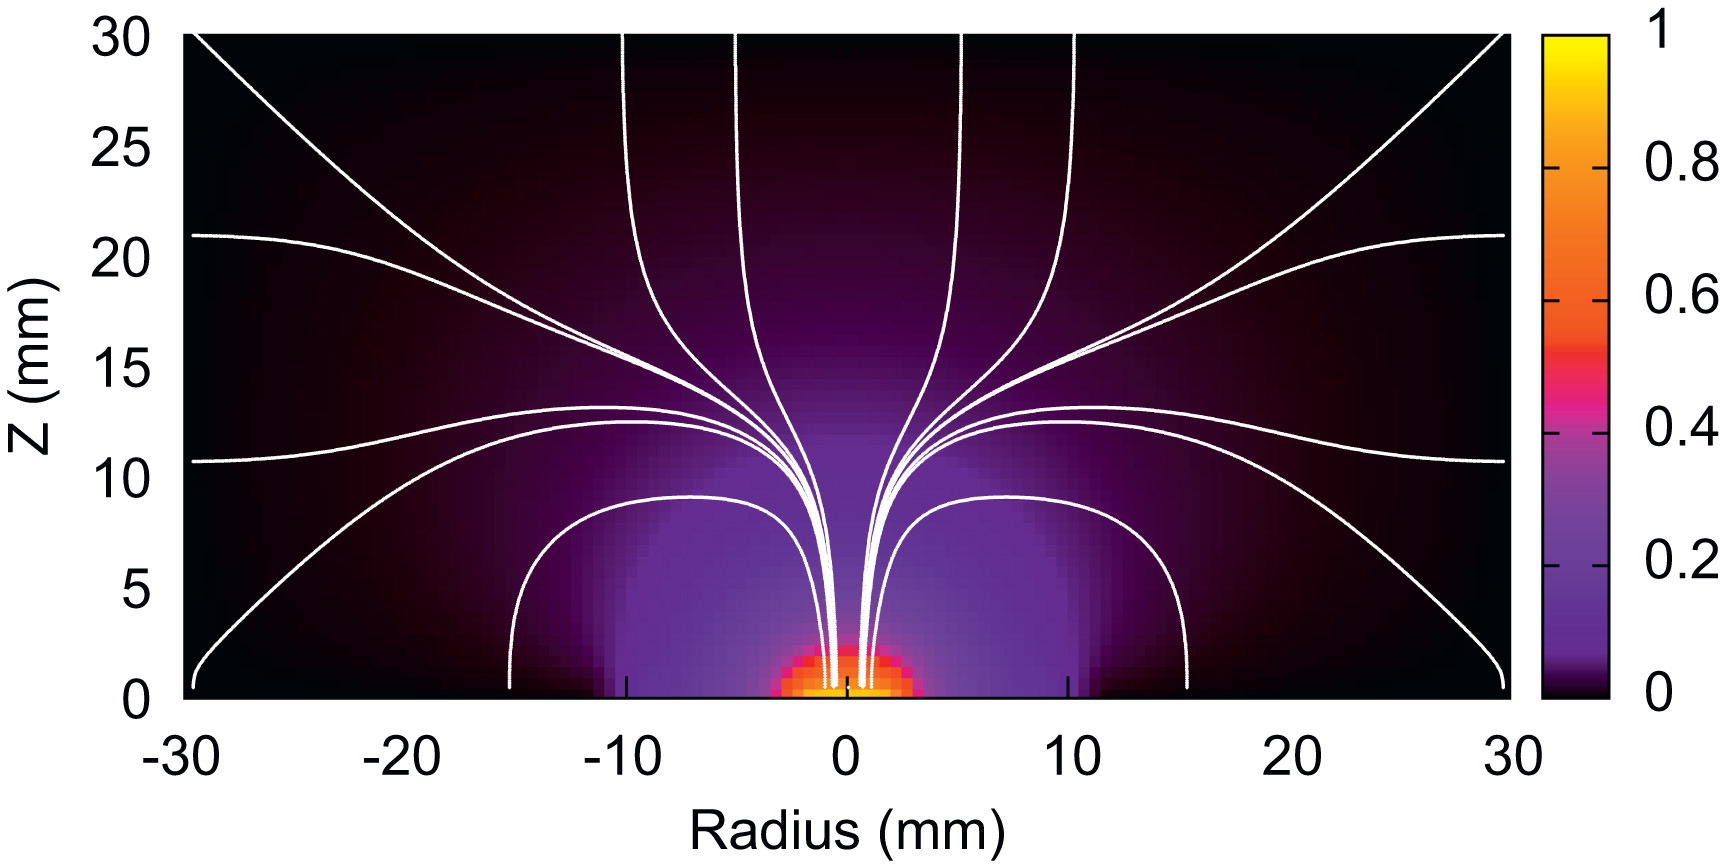
\includegraphics[width = .60\textwidth]{/Users/jgruszko/Documents/Thesis/Images/Ch1/PPCField.jpg} \hfil
\caption{A simulation of the weighting potential inside a PPC shows that charge drift paths (in white) are long and highly position-dependent. \cite{Aalseth2011}}
\label{PPCField}
\end{figure}

\subsection{PPCs and Low-Energy Recoils}
Because of their low thresholds and high masses, PPCs are a promising technology for low-mass WIMP searches and coherent neutrino-nuclear scattering experiments. The MALBEK and CoGeNT experiments are both low-background single-PPC experiments that have set competitive limits on (and in the case of CoGeNT, claimed observation of a signal consistent with) low-mass WIMPs \cite{MALBEK2015}\cite{COGENT2011}. One previous attempt was made to measure neutrino-nuclear scattering with a PPC \cite{BarbeauThesis}, and the COHERENT collaboration is currently considering using the technology for a future experiment at the Spallation Neutron Source \cite{CoherentSnowmassWP}. 

\subsection{Low-Energy Backgrounds in PPC Detectors}
As the tension between the MALBEK and CoGeNT results demonstrates, these measurements rely on a detailed understanding of background events near the detector threshold. Understanding these events, particularly from x-ray and $\alpha$ particle interactions, is the focus of this thesis. $\alpha$ events are also of great concern to the \MJ~ collaboration, as radon deposition on detector surfaces could contribute to backgrounds at the $0\nu\beta\beta$ Q-value. Though these backgrounds have been studied in N-type coaxial detectors \cite{JohnsonThesis2010}, this work is the first attempt to evaluate them in PPCs.